\chapter{Discussion}





The Ecological fallacy refers to inference about individuals based on analyses of group data. In such instance, individual characteristic are masked by the group average and it becomes harder to distinguish individual characteristics \citep{herring2001culture}. The same 






\section{1 stage Hierarchiacl Poisson model}

	\begin{equation}\nonumber
	y \sim Poisson(\mu) \;\;\; then \;\;\; E(y) = var(y) =\mu
	\end{equation}
	
	JAGS code




\section{2 stage Hierarchiacl Poisson model}

	\begin{equation}\nonumber
	y_T \sim Poisson(\sum_{i=1}^{N_i} \mu_i) 
	\end{equation}

	\begin{equation}\nonumber
	y_i \sim Poisson(\mu_i) 
	\end{equation}

	\begin{equation}\nonumber
	\mu_i \sim Gamma(\alpha,\beta) 
	\end{equation}

	Prior for the hyperparameters

	\begin{equation}\nonumber
	\alpha \sim Gamma(a,b) 
	\end{equation}

	\begin{equation}\nonumber
	\beta \sim Gamma(c,d) 
	\end{equation}
	
\section{3 stage Hierarchiacl Poisson model}

	\begin{equation}\nonumber
	y_T \sim Poisson(\sum_{i=1}^{N_i} \sum_{j=1}^{N_j}\mu_{ij}) 
	\end{equation}

	\begin{equation}\nonumber
	y_i \sim Poisson( \sum_{j=1}^{N_j}\mu_{j}) 
	\end{equation}
	
	\begin{equation}\nonumber
	y_{ij} \sim Poisson(\mu_{ij}) 
	\end{equation}

	\begin{equation}\nonumber
	\mu_{ij} \sim Gamma(\alpha,\beta) 
	\end{equation}

	Prior for the hyperparameters

	\begin{equation}\nonumber
	\alpha \sim Gamma(a_{ij},b_{ij}) 
	\end{equation}

	\begin{equation}\nonumber
	\beta \sim Gamma(c_{ij},d_{ij}) 
	\end{equation}
	
	Prior for the hyper-hyperparameters

	\begin{equation}\nonumber
	\alpha \sim Gamma(a_{ij},b_{ij}) 
	\end{equation}

	\begin{equation}\nonumber
	\beta \sim Gamma(c_{ij},d_{ij}) 
	\end{equation}

Notes

\begin{equation*}
y_i = \{y_A,y_B\}
\end{equation*}

\begin{equation*}
y_{ij} = \{y_{AA},y_{AB},y_{BA},y_{BB}\}
\end{equation*}

\begin{equation*}
\beta \sim Gamma(c_{ij},d_{ij}) 
\end{equation*}

\begin{equation*}
y_{t}=y_{AA,t}+y_{AB,t}+y_{BA,t}+y_{BB,t}.
\end{equation*}

\begin{equation*} y_{A,t}=y_{AA}{t}+y_{AB,t}\quad \quad y_{B,t}=y_{BA,t}+y_{BB,t}
\tag{10.4}
\end{equation*}

\section{Hierarchical Poisson regression models}
\section{Hierarchical timeseries models}


\section{Hierarchical Poisson timeseries models}


\begin{equation*}
\end{equation*}


\begin{figure}[!h]
	\centering
	\begin{tabular}{cc}
		\subf{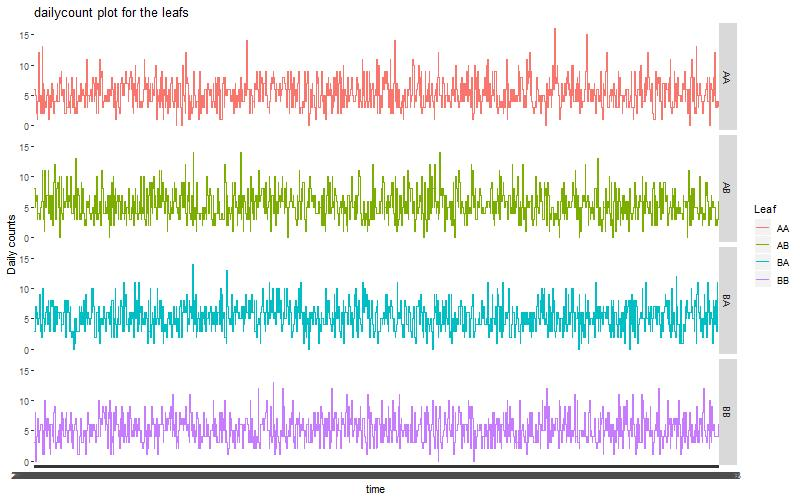
\includegraphics[width=65mm]{../../R-codes/Simulation/plot/anomaly/ggdaily1S10leaf}}
		{Anomaly$=10$}
		&
		\subf{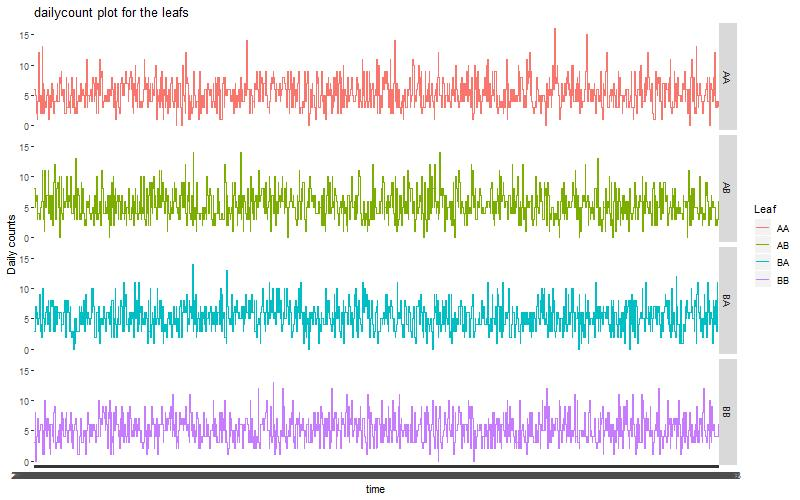
\includegraphics[width=65mm]{../../R-codes/Simulation/plot/anomaly/ggdaily1S25leaf}}
		{Anomaly$=2$}
		\\
		\subf{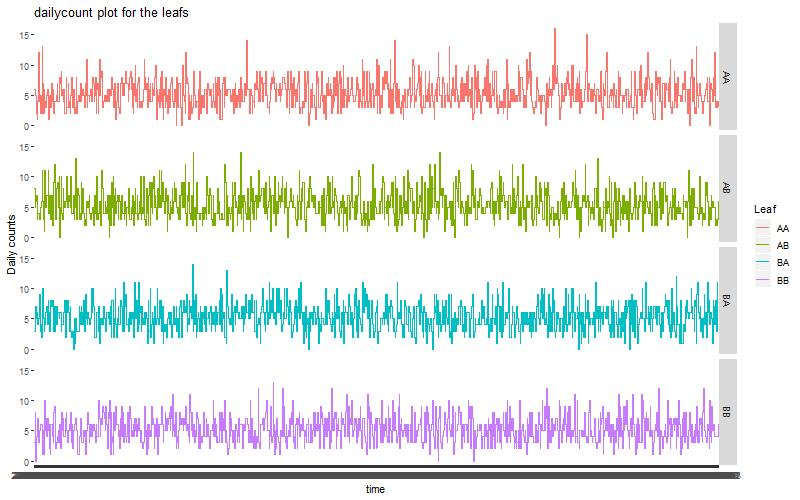
\includegraphics[width=65mm]{../../R-codes/Simulation/plot/anomaly/ggdaily1S50leaf}}
		{Anomaly$=50$}
		&
		\subf{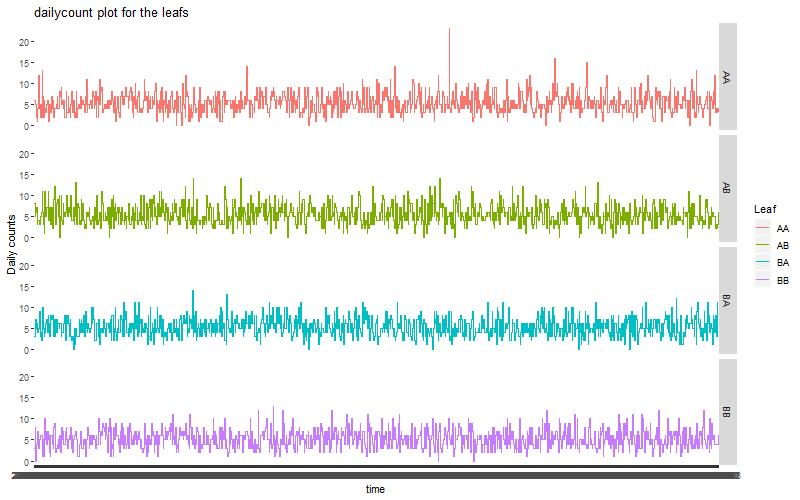
\includegraphics[width=65mm]{../../R-codes/Simulation/plot/anomaly/ggdaily1S100leaf}}
		{Anomaly$=100$}
		\\
		\subf{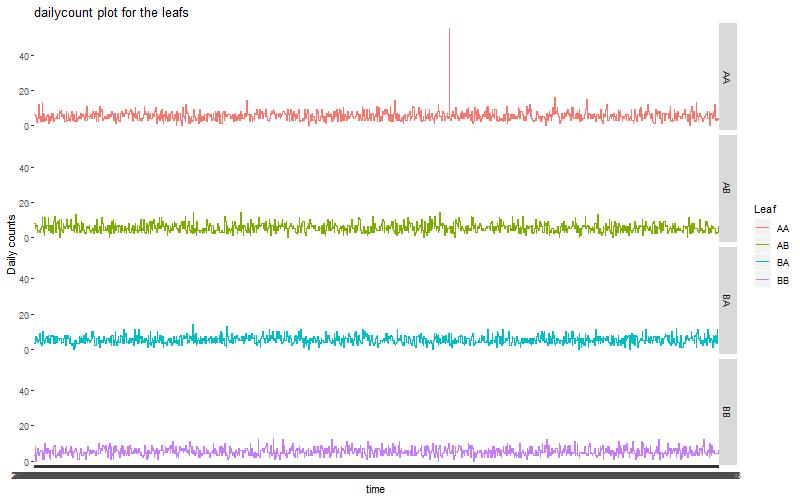
\includegraphics[width=65mm]{../../R-codes/Simulation/plot/anomaly/ggdaily1S250leaf}}
		{Anomaly'$=250$}
		&
		\subf{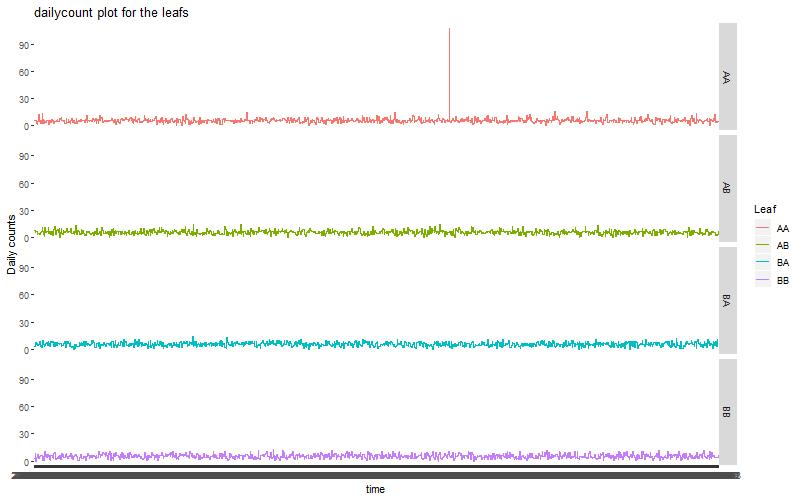
\includegraphics[width=65mm]{../../R-codes/Simulation/plot/anomaly/ggdaily1S500leaf}}
		{Anomaly $=500$}
		\\
	\end{tabular}
	\caption{Visual inspection of different increment of anomalies at level 2 of hierarchy}
	\label{fig:addanomleaf}
\end{figure}

\newpage %------------------------------------------------------------------------------------------    
\begin{figure}[!h]
	\centering
	\begin{tabular}{cc}
		\subf{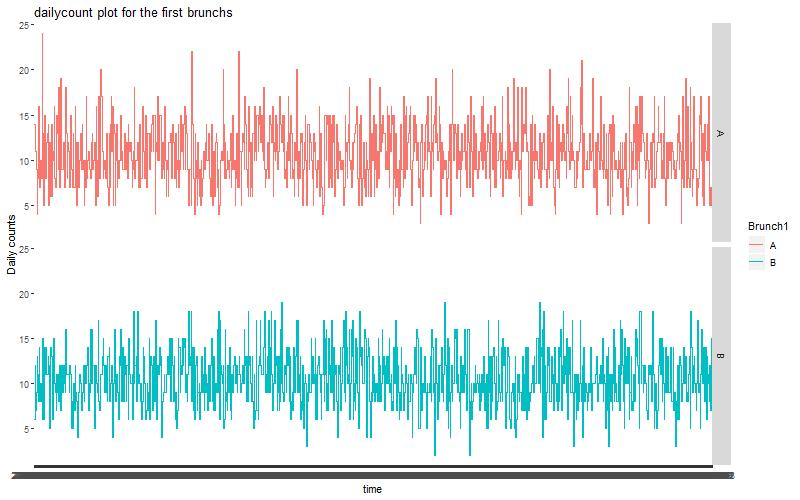
\includegraphics[width=65mm]{../../R-codes/Simulation/plot/anomaly/ggdaily1S10B1}}
		{Anomaly$=10$}
		&
		\subf{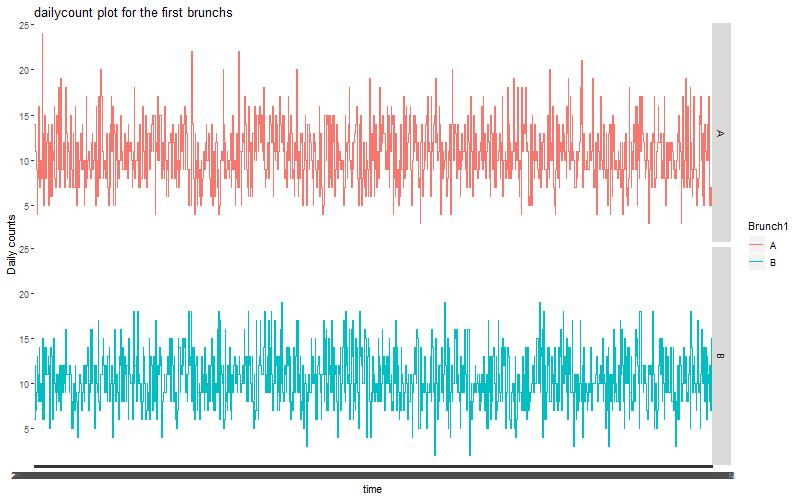
\includegraphics[width=65mm]{../../R-codes/Simulation/plot/anomaly/ggdaily1S25B1}}
		{Anomaly$=2$}
		\\
		\subf{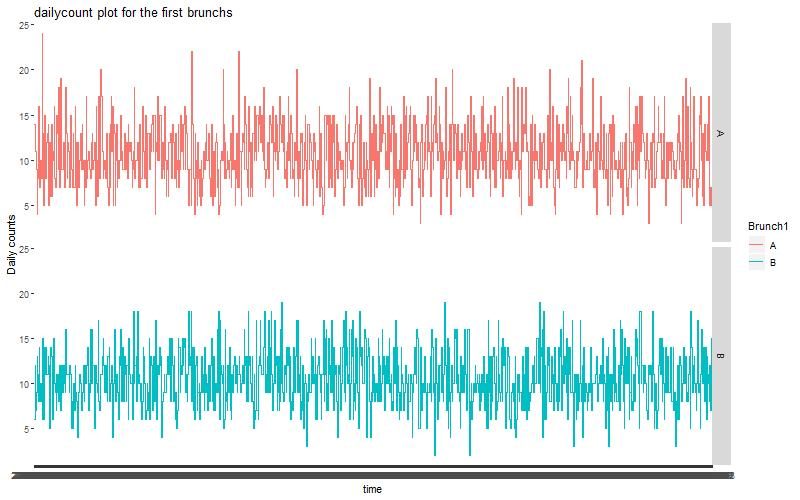
\includegraphics[width=65mm]{../../R-codes/Simulation/plot/anomaly/ggdaily1S50B1}}
		{Anomaly$=50$}
		&
		\subf{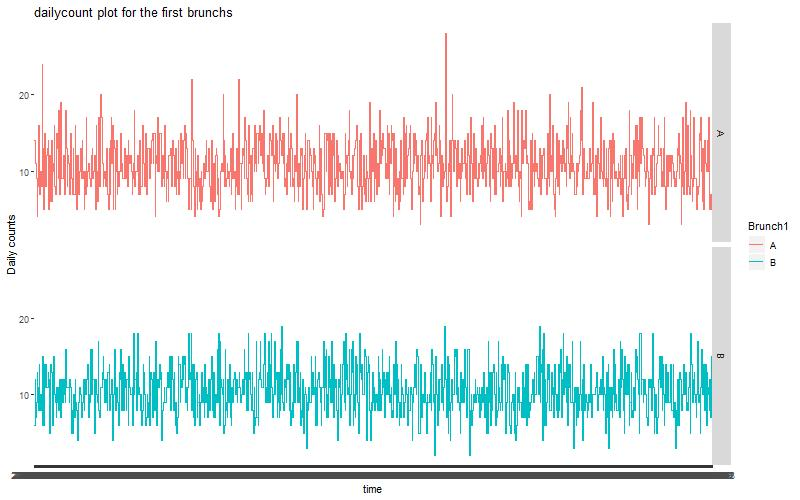
\includegraphics[width=65mm]{../../R-codes/Simulation/plot/anomaly/ggdaily1S100B1}}
		{Anomaly$=100$}
		\\
		\subf{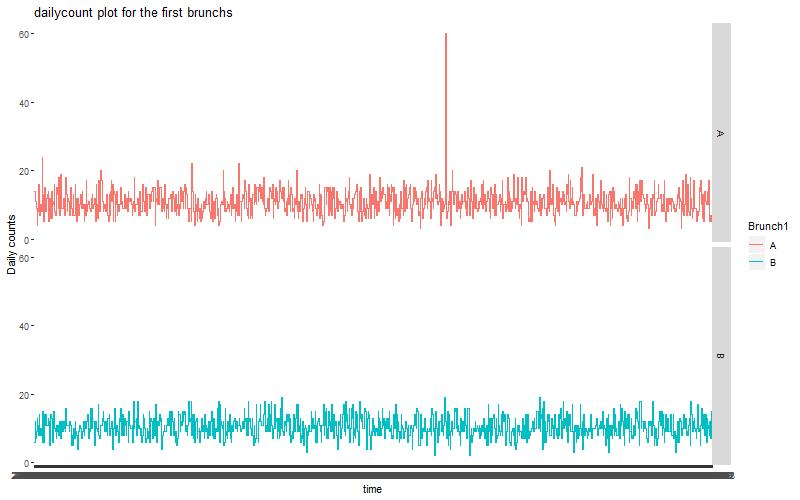
\includegraphics[width=65mm]{../../R-codes/Simulation/plot/anomaly/ggdaily1S250B1}}
		{Anomaly'$=250$}
		&
		\subf{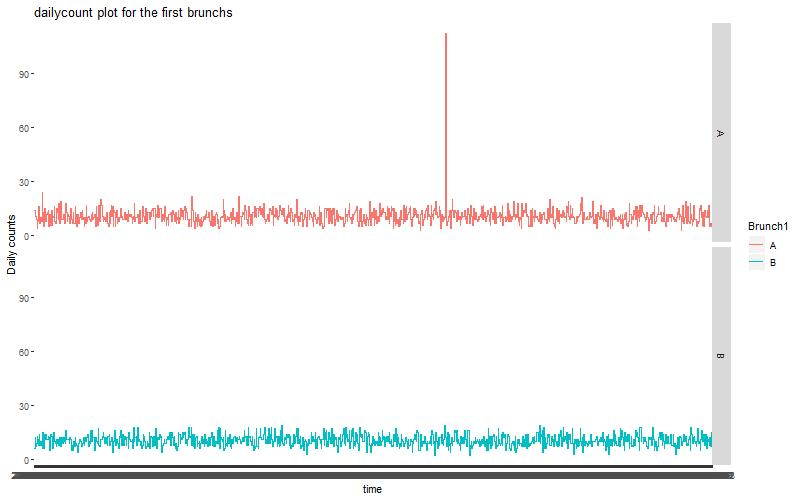
\includegraphics[width=65mm]{../../R-codes/Simulation/plot/anomaly/ggdaily1S500B1}}
		{Anomaly $=500$}
		\\
	\end{tabular}
	\caption{Visual inspection of different increment of anomalies at level 1 of hierarchy}
	\label{fig:addanomB1}
\end{figure}


